\documentclass{amsart}
\usepackage[margin=1in]{geometry}

\usepackage{amsmath, amssymb, latexsym}
\usepackage{tikz}
\usepackage{tikz-cd}
\usepackage{pgflibraryarrows}
\usepackage{pgflibrarysnakes}

\usepackage[draft]{say}
\newcommand{\sayER}[1]{\say[ER]{\color{blue}{\bf ER:}\;#1}}
\newcommand{\sayDR}[1]{\say[DR]{\color{red}{\bf DR:}\;#1}}

\newtheorem{theorem}{Theorem}
\newtheorem{example}[theorem]{Example}
\newtheorem{lemma}[theorem]{Lemma}
\newtheorem{remark}[theorem]{Remark}

\numberwithin{equation}{section}

\newcommand{\CC}{\mathbb{C}}
\newcommand{\PP}{\mathbb{P}}
\newcommand{\ZZ}{\mathbb{Z}}
\newcommand{\Hom}{\operatorname{Hom}}
\newcommand{\Span}{\operatorname{span}}
\newcommand{\bfe}{\mathbf{e}}
\newcommand{\bff}{\mathbf{f}}
\newcommand{\bfg}{\mathbf{g}}
\newcommand{\udim}{\underline{\dim}\,}

\newcommand{\into}{\hookrightarrow}

\title{2-Kronecker Quiver Grassmannians}
\author{Ed Richmond}
\author{Dylan Rupel}

\begin{document}
  \maketitle

  \section{Introduction}
  Quiver Grassmannians are projective varieties parametrizing subrepresentations of a given quiver representation.
  This gives a direct generalization of the standard Grassmannians of linear subspaces in a vector space but where the geometry behind linear transformations between such linear spaces is taken into consideration.
  Our goal in this project is to begin making explicit the geometry of these spaces.
  Unfortunately, in such an endeavor, it would be hopeless to expect a uniform description of this geometry since every projective variety can be realized as an appropriate quiver Grassmannian \cite{reineke}.
  
  We therefore restrict in this note to the well-studied example of the Kronecker quiver with two vertices and two parallel arrows as an initial proof of concept.
  In a subsequent work, we will utilize the results of \cite{rupel-weist} to extend our approach here to the Grassmannians of subrepresentations for the directly generalized $n$-Kronecker quivers (with an arbitrary number $n$ of parallel arrows between the pair of vertices); this simple case is already rich enough to encode the geometry of arbitrary projective varieties and so we restrict there and here to certain special representations with a more uniform geometric structure.

  In the 2-Kronecker case, we further restrict to the case of indecomposable representations, though with the help of Caldero-Chapoton fibrations (c.f. Section~\ref{???}) this restriction is easily removed.
  These quiver Grassmannians have been extensively studied, in the process of constructing our main results we reproduce the cell decompositions obtained by Cerulli Irelli and Esposito \cite{cerulli irelli-esposito}, albeit using very different methods which allow us to deduce an explicit description of the closures of these affine cells as unions of such cells.

  Our approach builds from the explicit description of Pl\"ucker relations for quiver Grassmannians developed by Lorscheid and Weist \cite{lorscheid-weist} which we utilize to give an explicit parametrization of the affine cells in such cell decompositions.
  This provides the essential tool we will use for understanding cell closures.

  \section{Pl\"ucker Coordinate Parametrization of Standard Schubert Cells}
  ToDo: Describe Pl\"ucker embedding of Grassmannians

  \section{Representations of the 2-Kronecker Quiver}

  Let $Q=1\substack{\longleftarrow\\\longleftarrow} 2$ be the 2-Kronecker quiver with arrows $Q_1=\{\alpha,\beta\}$.
  Write $W=\langle\alpha,\beta\rangle$ for the free group generated by the arrows of $Q$.
  There is a natural involution $\varphi$ of $W$ which interchanges the generators $\alpha$ and $\beta$.

  The \emph{universal covering quiver} $\widetilde Q$ of $Q$ is the quiver with vertex set $\widetilde Q_0=\{(i,w):i=1,2,\ w\in W\}$ and arrows $(\alpha,w):(2,w)\to(1,\alpha w)$ and $(\beta,w):(2,w)\to(1,\beta w)$ for $w\in W$.
  The automorphism $\varphi$ can be seen to act on $\widetilde Q_0$ via $\varphi\big((i,w)\big)=\big(i,\varphi(w)\big)$ for $i=1,2$ and on the arrows of $\widetilde Q$ via
  \[\varphi\big((\alpha,w)\big)=\big(\beta,\varphi(w)\big) \qquad \text{and} \qquad \varphi\big((\beta,w)\big)=\big(\alpha,\varphi(w)\big).\]
  We will only be interested in the two connected components of $\widetilde Q$ which are invariant under $\varphi$, namely those containing the vertices $(1,e)$ and $(2,e)$, where $e\in W$ is the identity element; these have the following forms:
  \[
    \begin{tikzcd}
      \widetilde Q^{(1)} := & \cdots & (1,\alpha\beta^{-1}) & & \fbox{$(1,e)$} & & (1,\beta\alpha^{-1}) & \cdots \\
      & \cdots \arrow["\beta"]{ur} & & (2,\beta^{-1}) \arrow["\alpha"']{ul} \arrow["\beta"]{ur} & & (2,\alpha^{-1}) \arrow["\alpha"']{ul} \arrow["\beta"]{ur} & & \cdots \arrow["\alpha"']{ul}
    \end{tikzcd}
  \]
  \[
    \begin{tikzcd}
      \hspace{-0.37cm} \widetilde Q^{(2)} := \hspace{0.37cm} & \cdots & & (1,\alpha) & & (1,\beta) & & \cdots \\
      & \cdots & (2,\beta^{-1}\alpha) \arrow["\alpha"']{ul} \arrow["\beta"]{ur} & & \fbox{$(2,e)$} \arrow["\alpha"']{ul} \arrow["\beta"]{ur} & & (2,\alpha^{-1}\beta) \arrow["\alpha"']{ul} \arrow["\beta"]{ur} & \cdots
    \end{tikzcd}
  \]
  The automorphism $\varphi$ then naturally acts on the categories of representations of $\widetilde Q^{(i)}$ for $i=1,2$.

  A representation $M$ of $Q$ consists of a pair of vector spaces $M_1,M_2$ together with a pair of linear maps $M_\alpha,M_\beta:M_2\to M_1$.
  The dimension vector of such a representation $M$ is the tuple $\udim M:=(\dim M_1,\dim M_2)$.

  We focus here on the indecomposable preprojective representations $P_k$ of $Q$ having the dimension vector $(k,k-1)$ for $k\ge1$.
  These admit several natural lifts to $\widetilde Q$ which will be useful.
  The first, denoted $\widetilde P_k$, are invariant under $\varphi$ and have the following forms with $k$ copies of $\CC$ in the top row:
  \[
    \text{k odd: }
    \begin{tikzcd}
      \cdots & & \CC & \cdots & & \fbox{$\CC$} & & \cdots & \CC & & \cdots \\
      \cdots & 0 \arrow["\alpha"']{ul} \arrow["\beta"]{ur} & & \cdots \arrow["\alpha"']{ul} & \CC \arrow["\alpha"']{ul} \arrow["\beta"]{ur} & & \CC \arrow["\alpha"']{ul} \arrow["\beta"]{ur} & \cdots \arrow["\beta"]{ur} & & 0 \arrow["\alpha"']{ul} \arrow["\beta"]{ur} & \cdots
    \end{tikzcd}
  \]
  \[
    \text{k even: }
    \begin{tikzcd}
      \cdots & & \CC & \cdots & \CC & & \CC & \cdots & \CC & & \cdots \\
      \cdots & 0 \arrow["\alpha"']{ul} \arrow["\beta"]{ur} & & \cdots \arrow["\alpha"']{ul} \arrow["\beta"]{ur} & & \fbox{$\CC$} \arrow["\alpha"']{ul} \arrow["\beta"]{ur} & & \cdots \arrow["\alpha"']{ul} \arrow["\beta"]{ur} & & 0 \arrow["\alpha"']{ul} \arrow["\beta"]{ur} & \cdots
    \end{tikzcd}
  \]
  where:
  \begin{itemize}
    \item for $k$ odd, $P_k$ lifts to a representation $\widetilde P_k$ supported on $\widetilde Q^{(1)}$;
    \item for $k$ even, $P_k$ lifts to a representation $\widetilde P_k$ supported on $\widetilde Q^{(2)}$.
  \end{itemize}

  These choices of lift to $\widetilde Q$ induces a basis $\{v_{k,1},\cdots,v_{k,2k-1}\}$ of $P_k$ such that for $t$ even $\alpha(v_{k,t})=v_{k,t-1}$ and $\beta(v_{k,t})=v_{k,t+1}$, i.e.\ we have the identifications
  \[P_{k,1}=\CC^k=\Span\{v_{k,t}:\text{$t$ odd}\}\qquad\text{and}\qquad P_{k,2}=\CC^{k-1}=\Span\{v_{k,t}:\text{$t$ even}\}.\]

  Write $\widetilde P_k^{(\alpha)}$ and $\widetilde P_k^{(\beta)}$ for the representations of $\widetilde Q$ obtained from $\widetilde P_k$ by the action of $\alpha$ and $\beta$ respectively.
  Note that these are naturally considered as subrepresentations of $\widetilde P_{k+1}$ and these are the only lifts of $\widetilde P_k$ with this property.
  \begin{lemma}
    \[\dim\Hom(P_k,P_{k+1})=2\]
  \end{lemma}

  For $\bfe=(e_1,e_2)\in\ZZ_{\ge0}^2$, write $Gr_\bfe(P_k)$ for the smooth projective variety of subrepresentations of $P_k$ with dimension vector $\bfe$.
  Note that $Gr_\bfe(P_k)$ is naturally considered as a closed subvariety of the product $Gr_{e_1}(\CC^k)\times Gr_{e_2}(\CC^{k-1})$.
  We aim to understand the geometry of these \emph{quiver Grassmannians} $Gr_\bfe(P_k)$.
  Our main observation is that the basis of $P_k$ induced by its lift $\widetilde P_k$ to the universal cover of $Q$ provides a reasonable compatibility between the geometry of $Gr_\bfe(P_k)$ and the associated standard Schubert decomposition of $Gr_{e_1}(\CC^k)\times Gr_{e_2}(\CC^{k-1})$.

  \section{Cell Decompositions}
  Here we describe two approaches to parametrizing the affine cells in a cell decomposition of $Gr_\bfe(P_k)$.
  Unfortunately, neither of these descriptions offers a transparent avenue for computing closures of cells.
  However, each one points to important ideas needed in our study.

  \subsection{Description via Torus Actions}
  The results of this section can be found in \cite{cerulli irelli-esposito}, we give an independent presentation for convenience of the reader and to introduce useful notation.

  Define a $\CC^*$-action on $P_k$ by $z.v_{k,t}=z^{-t}v_{k,t}$ for $t\in[1,2k-1]$.
  \begin{lemma}
    This induces a $\CC^*$-action on $Gr_\bfe(P_k)$.
    The fixed points of this action are precisely those subrepresentations of $P_k$ induced by subrepresentations of its lift $\widetilde P_k$ to the universal cover of $Q$.
    These in turn are naturally in bijection with successor-closed subsets of the support quiver of $\widetilde P_k$ with $e_1$ sink vertices and $e_2$ source vertices.
  \end{lemma}
  \begin{proof}
    The $\CC^*$-action on $P_k$ induces an action on $Gr_{e_1}(\CC^k)\times Gr_{e_2}(\CC^{k-1})$, we claim that $Gr_\bfe(P_k)\subseteq Gr_{e_1}(\CC^k)\times Gr_{e_2}(\CC^{k-1})$ is invariant under this action.
    Indeed, for $E\in Gr_\bfe(P_k)$ and $x_2\in E_2$, we may write $x_2=\sum\limits_{\text{$t$ even}} c_t v_{k,t}$.
    Then for $z\in\CC^*$, we have 
    \[\alpha(z.x_2)=\sum\limits_{\text{$t$ even}} c_t \alpha(z.v_{k,t})=\sum\limits_{\text{$t$ even}} c_t z^{-t}\alpha(v_{k,t})=z^{-1}\sum\limits_{\text{$t$ even}} c_t z.\alpha(v_{k,t})=z^{-1} \big(z.\alpha(x_2)\big)\in z.E_1\]
    with a similar calculation holding for $\beta$.
    This gives the first claim that $Gr_\bfe(P_k)$ is stable under the action.

    A point of $Gr_{e_1}(\CC^k)\times Gr_{e_2}(\CC^{k-1})$ is fixed by the $\CC^*$-action precisely when it consists of a pair $(E_1,E_2)$ of coordinate subspaces (with respect to the basis $\{v_{k,t}\}$ of $P_k$), i.e.\ they are described combinatorially via a pair of subsets $S_1\subseteq\{1\le t\le 2k-1:\text{$t$ odd}\}$ and $S_2\subseteq\{1\le t\le 2k-1:\text{$t$ even}\}$.
    In particular, these pairs naturally give rise to representations of $\widetilde Q$.
    Such a pair gives a fixed point inside $Gr_\bfe(P_k)$ precisely when it defines a subrepresentation of $P_k$, namely when $\alpha(E_2),\beta(E_2)\subseteq E_1$, or combinatorially when $\{t-1,t+1:t\in S_2\}\subseteq S_1$, that is when this determines a subrepresentation of $\widetilde P_k$.

    The combinatorial condition above is precisely the condition of being a successor-closed subset of the support quiver of $\widetilde P_k$.
  \end{proof}
  
  Write $E_{S_1,S_2}\in Gr_\bfe(P_k)$ for the fixed point associated to the successor-closed subset $S_1\sqcup S_2$ of the support quiver of $\widetilde P_k$.
  The \emph{attractor cell} of this fixed point is the set $A_{S_1,S_2}:=\{ E\in Gr_\bfe(P_k) : \lim\limits_{z\to 0} z.E=E_{S_1,S_2} \}$.
  More precisely, we may parametrize $A_{S_1,S_2}$ as the set of subrepresentations $E\subseteq P_k$ having the following form:
  \[ E_2 = \Span\{x_{k,t}:t\in S_2, x_{k,t}\in v_{k,t}+\bigoplus\limits_{\substack{t'<t\\ \text{$t'$ even}\\ t'\notin S_2}} \CC v_{k,t'} \} \]
  and
  \[ E_1 = \big(\alpha(E_2)+\beta(E_2)\big)\oplus\Span\{x_{k,t}:t\in S_1\setminus(\alpha(S_2)\cup\beta(S_2)), x_{k,t}\in v_{k,t}+\bigoplus\limits_{\substack{t'<t\\ \text{$t'$ odd}\\ t'\notin S_1}} \CC v_{k,t'} \}. \]
  Since the fixed points are isolated, we may apply the results of Bia\l{}ynicki-Birula to get a decomposition of $Gr_\bfe(P_k)$ into the affine spaces $A_{S_1,S_2}$, i.e.\ we have the decomposition 
  \[Gr_\bfe(P_k)=\bigsqcup_{S_1\sqcup S_2} A_{S_1,S_2}.\]
  Our goal is to compute the closures of the cells $A_{S_1,S_2}$ inside $Gr_\bfe(P_k)$.

  \begin{remark}
    The parametrization giving the subspaces $E_2$ inside $A_{S_1,S_2}$ is precisely the standard parametrization of the Schubert cell inside $Gr_{e_2}(\CC^{k-1})$ corresponding to the subset $S_2$.
  \end{remark}

  \subsection{Description of Cells via Tangent Spaces}
  \label{sec:tangent parametrization}
  The tangent space to $Gr_\bfe(P_k)$ at a point $E$ is naturally identified with the space $\Hom(E,P_k/E)$.
  If $E$ is a $\CC^*$-fixed point, there is an induced $\CC^*$-action on $\Hom(E,P_k/E)$.
  In this case, we may endow $\Hom(E,P_k/E)$ with a basis of eigenvectors for this action as follows.

  Let $S_1\sqcup S_2$ be a successor-closed subquiver of the support quiver of $\tilde P_k$ and $E_{S_1,S_2}\in Gr_\bfe(P_k)$ the corresponding $\CC^*$-fixed point.
  Since $S_1\sqcup S_2$ is successor-closed, it is not hard to see that the corresponding subquiver $\bar{S}_1\sqcup\bar{S}_2)$ is predecessor-closed for $\bar{S}_1:=\{1\le t\le 2k-1:\text{$t$ odd},t\notin S_1\}$ and $\bar{S}_2:=\{1\le t\le 2k-1:\text{$t$ even},t\notin S_2\}$.
  As can be seen in \cite[Prop. 2.0.2]{cerulli irelli-esposito}, the vector space $\Hom(E,P_k/E)$ admits a basis $\{f_\gamma\}$ labeled by isomorphisms $\gamma:\Gamma_E\to\Gamma_{P_k/E}$ from a connected predecessor-closed subquiver of $S_1\sqcup S_2$ to a connected successor-closed subquiver of $\bar{S}_1\sqcup\bar{S}_2$.

  Observe that the vertices of $\Gamma_E$ are of the form $v_{k,t},v_{k,t+1},\ldots$ for some $t\in[1,2k-1]$ and the vertices of $\Gamma_{P_k/E}$ are of the form $v_{k,t'},v_{k,t'+1},\ldots$ for some $t'\in[1,2k-1]$.
  The action of $\CC^*$ on the corresponding basis vector $f_\gamma$ of $\Hom(E,P_k/E)$ is given by
  \[z.f_\gamma=z^{t-t'}f_\gamma.\]

  \begin{lemma}
    Each attractor cell is isomorphic to the positive weight component of the tangent space of its fixed point.
  \end{lemma}

  Therefore, we may parametrize the attractor cell of a $\CC^*$-fixed point $E$ via the standard basis vectors $f_\gamma$ of $\Hom(E,P_k/E)$ for which $t>t'$, i.e. $\gamma$ represents a ``shift to the left'' in the support quiver of $\tilde P_k$.

  \begin{example}
    Let $k=9$ and consider the successor-closed subset $(S_1,S_2)$ of the support quiver of $\tilde P_k$ given by
    \[S_1=\{3,5,11,13,15,17\}\qquad\text{and}\qquad S_2=\{4,12,14\}\]
    \[
      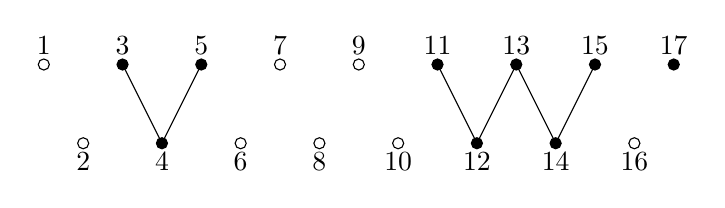
\begin{tikzpicture}
        \foreach \i in {3,5,11,13,15,17}{
          \draw[fill=black] (0.5*\i,1) circle (2pt);
          \node[above] at (0.5*\i,1) {\i};} 
        \foreach \i in {1,7,9}{
          \draw[fill=white] (0.5*\i,1) circle (2pt);
          \node[above] at (0.5*\i,1) {\i};} 
        \foreach \i in {4,12,14}{
          \draw[fill=black] (0.5*\i,0) circle (2pt);
          \draw (0.5*\i,0) -- (0.5*\i-0.5,1);
          \draw (0.5*\i,0) -- (0.5*\i+0.5,1);
          \node[below] at (0.5*\i,0) {\i};} 
        \foreach \i in {2,6,8,10,16}{
          \draw[fill=white] (0.5*\i,0) circle (2pt);
          \node[below] at (0.5*\i,0) {\i};} 
      \end{tikzpicture}
    \]
    The possible isomorphisms $\gamma$ with positive weight are given by
    \[
      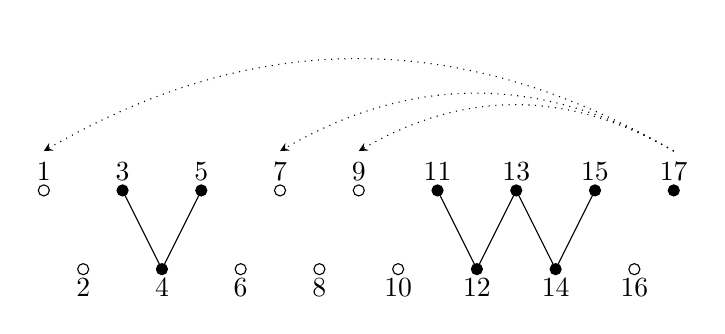
\begin{tikzpicture}
        \draw[dotted,-stealth] (8.5,1.5) to[out=150,in=30] (0.5,1.5);
        \draw[dotted,-stealth] (8.5,1.5) to[out=150,in=30] (3.5,1.5);
        \draw[dotted,-stealth] (8.5,1.5) to[out=150,in=30] (4.5,1.5);
        \foreach \i in {3,5,11,13,15,17}{
          \draw[fill=black] (0.5*\i,1) circle (2pt);
          \node[above] at (0.5*\i,1) {\i};} 
        \foreach \i in {1,7,9}{
          \draw[fill=white] (0.5*\i,1) circle (2pt);
          \node[above] at (0.5*\i,1) {\i};} 
        \foreach \i in {4,12,14}{
          \draw[fill=black] (0.5*\i,0) circle (2pt);
          \draw (0.5*\i,0) -- (0.5*\i-0.5,1);
          \draw (0.5*\i,0) -- (0.5*\i+0.5,1);
          \node[below] at (0.5*\i,0) {\i};} 
        \foreach \i in {2,6,8,10,16}{
          \draw[fill=white] (0.5*\i,0) circle (2pt);
          \node[below] at (0.5*\i,0) {\i};} 
      \end{tikzpicture}
    \]
    \[
      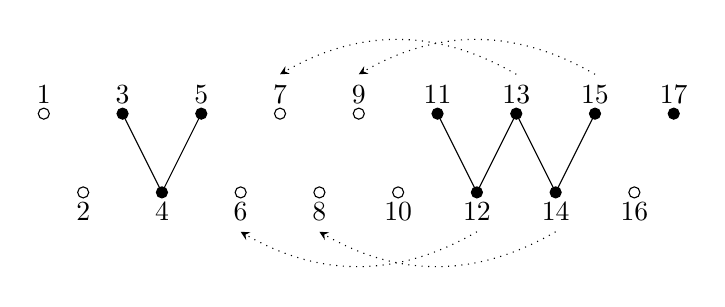
\begin{tikzpicture}
        \draw[dotted,-stealth] (6.5,1.5) to[out=150,in=30] (3.5,1.5);
        \draw[dotted,-stealth] (7.5,1.5) to[out=150,in=30] (4.5,1.5);
        \draw[dotted,-stealth] (6,-0.5) to[out=210,in=-30] (3,-0.5);
        \draw[dotted,-stealth] (7,-0.5) to[out=210,in=-30] (4,-0.5);
        \foreach \i in {3,5,11,13,15,17}{
          \draw[fill=black] (0.5*\i,1) circle (2pt);
          \node[above] at (0.5*\i,1) {\i};} 
        \foreach \i in {1,7,9}{
          \draw[fill=white] (0.5*\i,1) circle (2pt);
          \node[above] at (0.5*\i,1) {\i};} 
        \foreach \i in {4,12,14}{
          \draw[fill=black] (0.5*\i,0) circle (2pt);
          \draw (0.5*\i,0) -- (0.5*\i-0.5,1);
          \draw (0.5*\i,0) -- (0.5*\i+0.5,1);
          \node[below] at (0.5*\i,0) {\i};} 
        \foreach \i in {2,6,8,10,16}{
          \draw[fill=white] (0.5*\i,0) circle (2pt);
          \node[below] at (0.5*\i,0) {\i};} 
      \end{tikzpicture}
    \]
    \[
      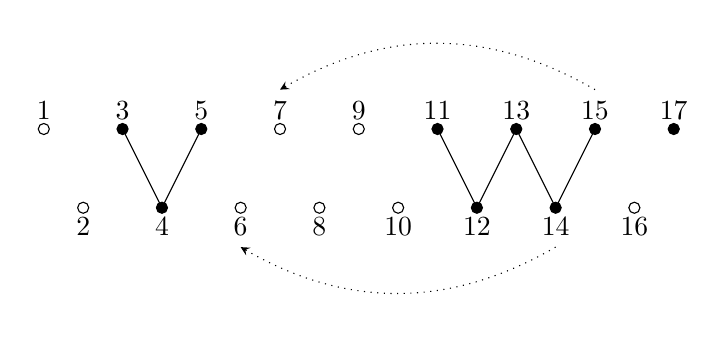
\begin{tikzpicture}
        \draw[dotted,-stealth] (7.5,1.5) to[out=150,in=30] (3.5,1.5);
        \draw[dotted,-stealth] (7,-0.5) to[out=210,in=-30] (3,-0.5);
        \foreach \i in {3,5,11,13,15,17}{
          \draw[fill=black] (0.5*\i,1) circle (2pt);
          \node[above] at (0.5*\i,1) {\i};} 
        \foreach \i in {1,7,9}{
          \draw[fill=white] (0.5*\i,1) circle (2pt);
          \node[above] at (0.5*\i,1) {\i};} 
        \foreach \i in {4,12,14}{
          \draw[fill=black] (0.5*\i,0) circle (2pt);
          \draw (0.5*\i,0) -- (0.5*\i-0.5,1);
          \draw (0.5*\i,0) -- (0.5*\i+0.5,1);
          \node[below] at (0.5*\i,0) {\i};} 
        \foreach \i in {2,6,8,10,16}{
          \draw[fill=white] (0.5*\i,0) circle (2pt);
          \node[below] at (0.5*\i,0) {\i};} 
      \end{tikzpicture}
    \]
    \[
      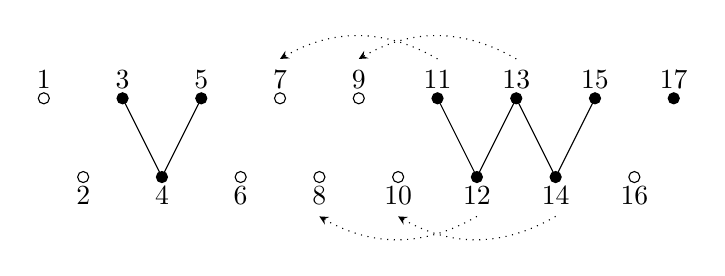
\begin{tikzpicture}
        \draw[dotted,-stealth] (5.5,1.5) to[out=150,in=30] (3.5,1.5);
        \draw[dotted,-stealth] (6.5,1.5) to[out=150,in=30] (4.5,1.5);
        \draw[dotted,-stealth] (6,-0.5) to[out=210,in=-30] (4,-0.5);
        \draw[dotted,-stealth] (7,-0.5) to[out=210,in=-30] (5,-0.5);
        \foreach \i in {3,5,11,13,15,17}{
          \draw[fill=black] (0.5*\i,1) circle (2pt);
          \node[above] at (0.5*\i,1) {\i};} 
        \foreach \i in {1,7,9}{
          \draw[fill=white] (0.5*\i,1) circle (2pt);
          \node[above] at (0.5*\i,1) {\i};} 
        \foreach \i in {4,12,14}{
          \draw[fill=black] (0.5*\i,0) circle (2pt);
          \draw (0.5*\i,0) -- (0.5*\i-0.5,1);
          \draw (0.5*\i,0) -- (0.5*\i+0.5,1);
          \node[below] at (0.5*\i,0) {\i};} 
        \foreach \i in {2,6,8,10,16}{
          \draw[fill=white] (0.5*\i,0) circle (2pt);
          \node[below] at (0.5*\i,0) {\i};} 
      \end{tikzpicture}
    \]
    \[
      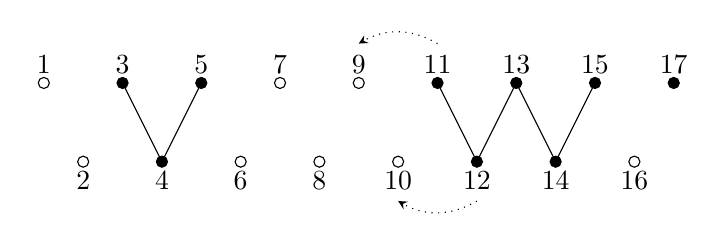
\begin{tikzpicture}
        \draw[dotted,-stealth] (5.5,1.5) to[out=150,in=30] (4.5,1.5);
        \draw[dotted,-stealth] (6,-0.5) to[out=210,in=-30] (5,-0.5);
        \foreach \i in {3,5,11,13,15,17}{
          \draw[fill=black] (0.5*\i,1) circle (2pt);
          \node[above] at (0.5*\i,1) {\i};} 
        \foreach \i in {1,7,9}{
          \draw[fill=white] (0.5*\i,1) circle (2pt);
          \node[above] at (0.5*\i,1) {\i};} 
        \foreach \i in {4,12,14}{
          \draw[fill=black] (0.5*\i,0) circle (2pt);
          \draw (0.5*\i,0) -- (0.5*\i-0.5,1);
          \draw (0.5*\i,0) -- (0.5*\i+0.5,1);
          \node[below] at (0.5*\i,0) {\i};} 
        \foreach \i in {2,6,8,10,16}{
          \draw[fill=white] (0.5*\i,0) circle (2pt);
          \node[below] at (0.5*\i,0) {\i};} 
      \end{tikzpicture}
    \]
    \[
      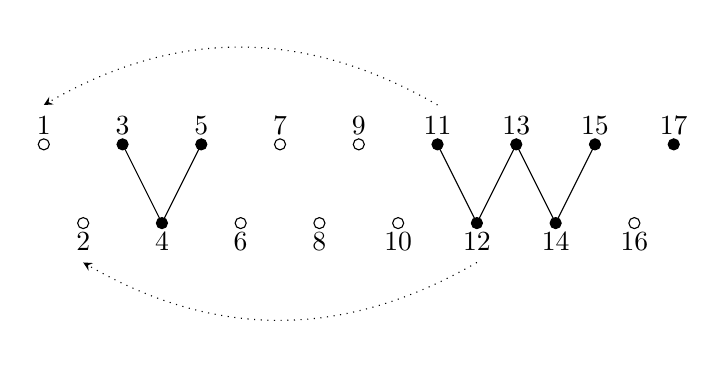
\begin{tikzpicture}
        \draw[dotted,-stealth] (5.5,1.5) to[out=150,in=30] (0.5,1.5);
        \draw[dotted,-stealth] (6,-0.5) to[out=210,in=-30] (1,-0.5);
        \foreach \i in {3,5,11,13,15,17}{
          \draw[fill=black] (0.5*\i,1) circle (2pt);
          \node[above] at (0.5*\i,1) {\i};} 
        \foreach \i in {1,7,9}{
          \draw[fill=white] (0.5*\i,1) circle (2pt);
          \node[above] at (0.5*\i,1) {\i};} 
        \foreach \i in {4,12,14}{
          \draw[fill=black] (0.5*\i,0) circle (2pt);
          \draw (0.5*\i,0) -- (0.5*\i-0.5,1);
          \draw (0.5*\i,0) -- (0.5*\i+0.5,1);
          \node[below] at (0.5*\i,0) {\i};} 
        \foreach \i in {2,6,8,10,16}{
          \draw[fill=white] (0.5*\i,0) circle (2pt);
          \node[below] at (0.5*\i,0) {\i};} 
      \end{tikzpicture}
    \]
    \[
      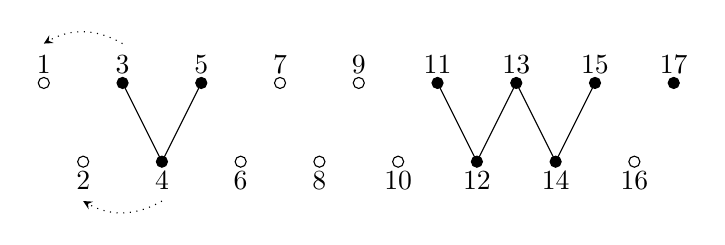
\begin{tikzpicture}
        \draw[dotted,-stealth] (1.5,1.5) to[out=150,in=30] (0.5,1.5);
        \draw[dotted,-stealth] (2,-0.5) to[out=210,in=-30] (1,-0.5);
        \foreach \i in {3,5,11,13,15,17}{
          \draw[fill=black] (0.5*\i,1) circle (2pt);
          \node[above] at (0.5*\i,1) {\i};} 
        \foreach \i in {1,7,9}{
          \draw[fill=white] (0.5*\i,1) circle (2pt);
          \node[above] at (0.5*\i,1) {\i};} 
        \foreach \i in {4,12,14}{
          \draw[fill=black] (0.5*\i,0) circle (2pt);
          \draw (0.5*\i,0) -- (0.5*\i-0.5,1);
          \draw (0.5*\i,0) -- (0.5*\i+0.5,1);
          \node[below] at (0.5*\i,0) {\i};} 
        \foreach \i in {2,6,8,10,16}{
          \draw[fill=white] (0.5*\i,0) circle (2pt);
          \node[below] at (0.5*\i,0) {\i};} 
      \end{tikzpicture}
    \]

  \end{example}

  \section{Quiver Pl\"ucker Coordinates}
  Given a totally ordered set $K$, write $\epsilon(k,K)=\#\{k'\in K: k'\le k\}$.

  Consider the embedding $Gr_\bfe(P_k)\into Gr_{e_1}(\CC^k)\times Gr_{e_2}(\CC^{k-1})\into \PP^{k \choose e_1}\times \PP^{k-1 \choose e_2}$ which is the composition of the natural inclusion $Gr_\bfe(P_k)\into Gr_{e_1}(\CC^k)\times Gr_{e_2}(\CC^{k-1})$ with the Pl\"ucker embeddings of the ordinary Grassmannians according to the basis $\{v_{k,1},\cdots,v_{k,2k-1}\}$ of $P_k$.
  Then $Gr_\bfe(P_k)$ may be described explicitly in terms of the Pl\"ucker coordinates 
  \[[\Delta_I:\Delta_J]_{I\subseteq_{e_1} \{1,3,\ldots,2k-1\}, J\subseteq_{e_2} \{2,4,\ldots,2k-2\}}.\]
  
  Indeed, since $Gr_\bfe(P_k)$ lies inside $Gr_{e_1}(\CC^k)\times Gr_{e_2}(\CC^{k-1})$, the ordinary Pl\"ucker relations must be satisfied:
  \[\sum_{i\in I'\setminus I} (-1)^{\epsilon(i,I)} \Delta_{I\cup\{i\}} \Delta_{I'\setminus\{i\}}=0
    \qquad
    \sum_{j\in J'\setminus J} (-1)^{\epsilon(j,J)} \Delta_{J\cup\{j\}} \Delta_{J'\setminus\{j\}}=0\]
  for each $I,I'\subseteq\{1,3,\ldots,2k-1\}$ with cardinalities $e_1-1,e_1+1$ respectively and each $J,J'\subseteq\{2,4,\ldots, 2k-2\}$ with cardinalities $e_2-1,e_2+1$ respectively.
  In addition, the \emph{quiver Pl\"ucker relations} must be satisfied \cite{lorscheid-weist}:
  \begin{align}
    \label{eq:left Plucker} \sum_{j\in \{2,4,\ldots,2k-2\}\setminus J} (-1)^{\epsilon(j-1,I)+\epsilon(j,J)} \Delta_{I\setminus\{j-1\}} \Delta_{J\cup\{j\}}=0,\\
    \label{eq:right Plucker} \sum_{j\in \{2,4,\ldots,2k-2\}\setminus J} (-1)^{\epsilon(j+1,I)+\epsilon(j,J)} \Delta_{I\setminus\{j+1\}} \Delta_{J\cup\{j\}}=0,
  \end{align}
  for each $I\subseteq\{1,3,\ldots,2k-1\}$ with cardinality $e_1+1$ and each $J\subseteq\{2,4,\ldots, 2k-2\}$ with cardinality $e_2-1$.
  In the equations above, we take $\Delta_I=0$ if $|I|=e_1+1$, i.e. when $j-1\notin I$ in \eqref{eq:left Plucker} or when $j+1\notin I$ in \eqref{eq:right Plucker}.
  \begin{remark}
    \label{rm:linear terms}
    Note that, upon restriction to an attractor cell $A_{S_1,S_2}$, each quiver Pl\"ucker relation has either zero, one, or two linear terms since the restriction imposes $\Delta_{S_1}=\Delta_{S_2}=1$.
    Thus necessary conditions for there to exist two linear terms are the containments $S_1\subseteq I$ and $J\subseteq S_2$.
    Moreover, this condition precludes the possibility that a constant appears in a restricted quiver Pl\"ucker relation since $I\setminus\{j\pm1\}=S_1$ and $J\cup\{j\}=S_2$ are incompatible with the successor-closed requirement for the subquiver $S_1\sqcup S_2$ to label a cell in $Gr_\bfe(P_k)$.
  \end{remark}

  \begin{lemma}
    Let $S_1\sqcup S_2$ be a successor-closed subset of the support quiver of $\tilde P_k$ with $|S_i|=e_i$.
    Given $I \subseteq_{e_1} \{1,3,\ldots,2k-1\}$ (resp. $J \subseteq_{e_2} \{2,4,\ldots, 2k-2\}$), we have $\Delta_I\equiv 0$ (resp. $\Delta_J\equiv 0$) when restricted to the attractor cell $A_{S_1,S_2}$ if there exists $t\in I\setminus S_1$ such that $\#\{s\in S_1:s\notin I, s>t\} < \#\{s\in I:s\notin S_1, s \ge t\}$ (and similarly for $J$).
  \end{lemma}
  \begin{proof}
    This matches the same condition for vanishing of Pl\"ucker coordinates in ordinary Schubert cells.
  \end{proof}

  \begin{lemma}
    Let $S_1\sqcup S_2$ be a successor-closed subset of the support quiver of $\tilde P_k$ with $|S_i|=e_i$.
    Given $I \subseteq_{e_1} \{1,3,\ldots,2k-1\}$ (resp. $J \subseteq_{e_2} \{2,4,\ldots, 2k-2\}$) with $|I\setminus S_1|\ge2$ and $\Delta_I\not\equiv 0$ on $A_{S_1,S_2}$ (resp. $|J\setminus S_2|\ge 2$ and $\Delta_J\not\equiv 0$ on $A_{S_1,S_2}$), there exists a standard Pl\"ucker relation in which $\Delta_I$ (resp. $\Delta_J$) is the sole linear term.
    Moreover, in any such Pl\"ucker relation every other Pl\"ucker coordinate $\Delta_{I'}$ (resp. $\Delta_{J'}$) appearing in the relation satisfies $I<I'$ (resp. $J<J'$) in the reverse lexicographic ordering.
  \end{lemma}

  The following describes those quiver Pl\"ucker relations with two linear terms over $A_{S_1,S_2}$.
  \begin{lemma}
    Let $S_1\sqcup S_2$ be a successor-closed subset of the support quiver of $\tilde P_k$ with associated fixed point $E$ and $\bar{S}_1\sqcup\bar{S}_2$ the predecessor-closed subset associated with $P_k/E$.
    The subsets $I\subseteq\{1,3,\ldots,2k-1\}$ with cardinality $e_1+1$ and $J\subseteq\{2,4,\ldots, 2k-2\}$ with cardinality $e_2-1$ for which the quiver Pl\"ucker relation \eqref{eq:left Plucker} (resp. \eqref{eq:right Plucker}) has two linear terms are precisely those of the form
    \[I=S_1\cup\{\sigma_\ell(s-1)\} \qquad \text{and} \qquad J=S_2\setminus\{s\}\]
    (resp. $I=S_1\cup\{\sigma_\ell(s+1)\}$ and $J=S_2\setminus\{s\}$), where $s\in S_2$ and $\sigma_\ell(t)=t-\ell$ for $\ell\ge1$ with $\sigma_\ell(s)\in\bar{S}_2$ and $\sigma_\ell(s-1)\in\bar{S}_1$ (resp. $\sigma_\ell(s+1)\in\bar{S}_1$).
    In this case, quiver Pl\"ucker relation \eqref{eq:left Plucker} (resp. \eqref{eq:right Plucker}) contains the two linear terms $\Delta_{I\setminus\{s-1\}\cup\{\sigma_\ell(s-1)\}}$ (resp. $\Delta_{I\setminus\{s+1\}\cup\{\sigma_\ell(s+1)\}}$) and $\Delta_{J\setminus\{s\}\cup\{\sigma_\ell(s)\}}$.
  \end{lemma}
  \begin{proof}
    Observe first that indeed the quiver Pl\"ucker relations given above have two linear terms since $s\pm1\in S_1$ for $s\in S_2$ while the conditions on the shift $\ell$ imply $\sigma_\ell(s\pm1)\notin S_1$ and $\sigma_\ell(s)\notin S_2$ with $\Delta_{S_1\setminus\{s\pm1\}\cup\{\sigma_\ell(s\pm1)\}}$ and $\Delta_{S_2\setminus\{s\}\cup\{\sigma_\ell(s)\}}$ not identically zero on $A_{S_1,S_2}$.

    Now consider subsets $I$ and $J$ with $S_1\subseteq I$ and $J\subseteq S_2$ for which a quiver Pl\"ucker relation \eqref{eq:left Plucker} or \eqref{eq:right Plucker} has two linear terms.
    Set $\varepsilon=-1$ if this relation comes from \eqref{eq:left Plucker} and set $\varepsilon=+1$ if this relation comes from \eqref{eq:right Plucker}.
    Let $t+\varepsilon$ denote the unique element in $I\setminus S_1$ and let $s$ denote the unique element in $S_2\setminus J$.
    By assumption, the term $\Delta_{I\setminus\{t+\varepsilon\}} \Delta_{J\cup\{t\}}$ must be linear and so the minor $\Delta_{J\cup\{t\}}$ cannot be identically zero nor identically one on $A_{S_1,S_2}$ following Remark~\ref{rm:linear terms}.
    This forces $t<s$ and $t\in\bar{S_2}$.
    Similar consideration with the term $\Delta_{I\setminus\{s+\varepsilon\}} \Delta_{J\cup\{s\}}$ show that $s+\varepsilon\in\bar{S}_1$.
    Thus we may set $\ell=s-t$ and construct the sets $I$ and $J$ as above.
  \end{proof}

  The next two results describe those quiver Pl\"ucker relations with only one linear term over $A_{S_1,S_2}$.
  \begin{lemma}
    Upon restriction to $A_{S_1,S_2}$, a minor $\Delta_I$ (resp. $\Delta_J$) is the sole linear term in a quiver Pl\"ucker relation if it is not identically zero on $A_{S_1,S_2}$ and differs from $S_1$ (resp. $S_2$) in at least two places.
  \end{lemma}
  \begin{lemma}
    \mbox{}
    \begin{enumerate}
      \item For every lift of an arrow of $Q$ to $S_1\sqcup S_2$ and to $\bar{S}_1\sqcup \bar{S}_2$, there exists a unique minimal expansion to a pair consisting of a connected predecessor-closed subquiver $\Gamma_E$ of $S_1\sqcup S_2$ and a connected successor-closed subquiver $\Gamma_{P_k/E}$ of $\bar{S}_1\sqcup \bar{S}_2$ each containing the respective lifted arrow with a corresponding (partial) isomorphism $\gamma:\Gamma_E\to\Gamma_{P_k/E}$.
      \item If the expansions $\Gamma_E$ and $\Gamma_{P_k/E}$ are not isomorphic quivers, then the following hold:
        \begin{enumerate}
          \item $1=\gamma(s+1)$ for some $s+1\in S_1$;
          \item $\gamma$ is surjective;
          \item the minor $\Delta_{S_1\setminus\{s+1\}\cup\{1\}}$ appears as the sole linear term in a quiver Pl\"ucker relation, where $s+1$ is the vertex of $\Gamma_E$ identified with vertex $1$ of $\Gamma_{P_k/E}$ under the bijection of vertices coming from the expansion procedure;
          \item none of the minors associated to $\gamma$ are necessary to parametrize the cell $A_{S_1,S_2}$.
        \end{enumerate}
    \end{enumerate}
  \end{lemma}
  \begin{proof}
    Take $I=S_1\cup\{1\}$ and $J=S_2\setminus\{s\}$ in the quiver Pl\"ucker relation \eqref{eq:right Plucker}.
  \end{proof}

  \begin{lemma}
    Let $S_1\sqcup S_2$ be a successor-closed subset of the support quiver of $\tilde P_k$ with associated $\CC^*$-fixed point $E\in Gr_\bfe(P_k)$.
    Given any isomorphism $\gamma:\Gamma_E\to\Gamma_{P_k/E}$ as in Section~\ref{sec:tangent parametrization}, say with
    \[\Gamma_E=\{v_{k,t},v_{k,t+1},\ldots,v_{k,t+\ell}\}\qquad\text{and}\qquad\Gamma_{P_k/E}=\{v_{k,t'},v_{k,t'+1},\ldots,v_{k,t'+\ell}\}\]
    such that $t'<t$ and $\ell>0$, the following hold:
    \begin{enumerate}
      \item there exists a quiver Pl\"ucker relation which, upon restriction to $A_{S_1,S_2}$, takes the form
        \[\Delta_{S_1\setminus\{s-1\}\cup\{\gamma(s-1)\}}-\varepsilon_\gamma(s)\Delta_{S_2\setminus\{s\}\cup\{\gamma(s)\}}=homogeneous~quadratic\]
        whenever $s$ is even with $t<s\le t+\ell$;
      \item there exists a quiver Pl\"ucker relation which, upon restriction to $A_{S_1,S_2}$, takes the form
        \[\Delta_{S_1\setminus\{s+1\}\cup\{\gamma(s+1)\}}-\varepsilon'_\gamma(s)\Delta_{S_2\setminus\{s\}\cup\{\gamma(s)\}}=homogeneous~quadratic\]
        whenever $s$ is even with $t\le s<t+\ell$.
    \end{enumerate}
  \end{lemma}
  \begin{proof}
    Observe that $\Delta_{S_1}=\Delta_{S_2}=1$ on $A_{S_1,S_2}$.
    Take $I=S_1\cup\{\gamma(s-1)\}$ and $J=S_2\setminus\{s\}$ in equation \eqref{eq:left Plucker} for $s$ even with $t<s\le t+\ell$ to get part (1).
    Take $I=S_1\cup\{\gamma(s+1)\}$ and $J=S_2\setminus\{s\}$ in equation \eqref{eq:right Plucker} for $s$ even with $t\le s<t+\ell$ to get part (2).
  \end{proof}

  \begin{lemma}
    Let $S_1\sqcup S_2$ be a successor-closed subset of the support quiver of $\tilde P_k$ with associated fixed point $E$.
    There exists $I\subseteq\{1,3,\ldots,2k-1\}$ with cardinality $e_1+1$ and each $J\subseteq\{2,4,\ldots, 2k-2\}$ with cardinality $e_2-1$ such that $S_1\subseteq I$ and $J\subseteq S_2$ if and only if 
  \end{lemma}
  
  \begin{theorem}
    Let $S_1\sqcup S_2$ be a successor-closed subset of the support quiver of $\tilde P_k$ with $|S_i|=e_i$.
    Then the attractor cell $A_{S_1,S_2}$ is parametrized as an affine space by the Pl\"ucker coordinates 
    \begin{itemize}
      \item $\Delta_J$ for $J=S_2\setminus\{s\}\cup\{t\}$ with $s\in S_2$, $t\in\bar{S}_2$, and $t<s$;
      \item $\Delta_I$ for $I=???$
    \end{itemize}
  \end{theorem}
  \begin{proof}
    By construction, upon restriction to $A_{S_1,S_2}$ we have $\Delta_{S_1}\equiv 1$, $\Delta_{S_2}\equiv 1$.
    Also,
    \[\Delta_I\equiv 0 \qquad \Delta_J\equiv 0\]
    if there exists $i\in I\setminus S_1$ such that $\#\{j\in S_1:j\notin I, j>i\} < \#\{j\in I:j\notin S_1,j>i\}$ and similarly for $J$.
  \end{proof}

% \section{Approach 2: Caldero-Chapoton Fibrations}
% Given a short exact sequence 
% \[\begin{tikzcd}
%   0 \arrow{r} & M \arrow["\iota"]{r} & B \arrow["\pi"]{r} & N \arrow{r} & 0
% \end{tikzcd}\]
% of representations, we get an induced map of quiver Grassmannians
% \begin{align*}
%   \Psi:Gr_\bfe(B) &\to \bigsqcup_{\bff+\bfg=\bfe} Gr_\bff(M)\times Gr_\bfg(N) \\
%   E &\mapsto \big(E\cap\iota(M),\pi(E)=(E+\iota(M))/\iota(M)\big)
% \end{align*}
% A result of Caldero and Chapoton shows that the fiber over a point $(F,G)$ in the image of $\Psi$ is isomorphic to the affine space $\Hom_Q(G,M/F)$.

% The difficulty of using these maps to inductively establish cell decompositions of quiver Grassmannians is in understanding the how these fiber dimensions vary over the image of $\Psi$.
% In our situation, these can be controlled for special short exact sequences:
% \[\begin{tikzcd}
%     0 \arrow{r} & P_k^{\alpha} \arrow["\alpha"]{r} & P_{k+1} \arrow{r} & D_\beta \arrow{r} & 0
% \end{tikzcd}\]
% for $k$ odd, where the dimension vector of $D_\beta$ is $(1,1)$ with $\alpha$ acting as zero and $\beta$ acting as the identity map, and
% \[\begin{tikzcd}
%     0 \arrow{r} & P_k^{\beta} \arrow["\beta"]{r} & P_{k+1} \arrow{r} & D_\beta \arrow{r} & 0
% \end{tikzcd}\]
% for $k$ even.
% \begin{lemma}
%   For any proper subrepresentation $G\subsetneq D_\beta$ and any subrepresentation $F\subseteq P_k$, the fiber $\Psi^{-1}(F,G)$ is non-empty
% \end{lemma}


\begin{thebibliography}{10}

\bibitem{ass} 
  I.~Assem, D.~Simson, A.~Skowronski: Elements of the Representation Theory of Associative Algebras. Cambridge University Press, Cambridge 2007.

\bibitem{ars} 
  M.~Auslander, I.~Reiten, S.~O.~Smalo: Representation theory of Artin algebras {\bf 36}. Cambridge University Press, Cambridge 1997.

\bibitem{bb} 
  A.~Bia\l{}ynicki-Birula: Some theorems on actions of algebraic groups. Annals of Mathematics \textbf{98}, 480-497 (1973).

\bibitem{bgp} 
  I.~N.~Bernstein, I.~M.~Gelfand, V.~A.~Ponomarev: Coxeter functors, and Gabriel's theorem. Russian Mathematical Surveys \textbf{28}(2), 17-32 (1973).

\bibitem{brenner-butler} 
  S.~Brenner, M.~C.~R.~Butler: The equivalence of certain functors occurring in the representation theory of artin algebras and species. Journal of the London Mathematical Society \textbf{2}(1), 183-187 (1976).

\bibitem{cc} 
  P.~Caldero, F.~Chapoton: Cluster algebras as {H}all algebras of quiver representations. Commentarii Mathematici Helvetici \textbf{81}(3), 595-616 (2006).

\bibitem{ck} 
  P.~Caldero, B.~Keller: From triangulated categories to cluster algebras II.  Annales Scientifique de l'Ecole Normale Superi\'{e}ure (4) \textbf{39} (6), 983-1009 (2006).

\bibitem{cr} 
  P.~Caldero, M.~Reineke: On the quiver Grassmannian in the acyclic case. Journal of Pure and Applied Algebra \textbf{212}(11), 2369-2380 (2008).

\bibitem{ca}	J.B.~Carrell: Torus actions and cohomology. Algebraic quotients. Torus actions and cohomology. The adjoint representation and the adjoint action, 83-158. Encyclopaedia Mathematical Science \textbf{131}, Invariant Theory and Algebraic Transformation Groups, Springer, Berlin, 2002.

\bibitem{cerulli irelli-esposito} 
  G.~Cerulli Irelli, F.~Esposito: Geometry of quiver Grassmannians of Kronecker type and applications to cluster algebras. Algebra \&  Number Theory \textbf{5}(6), 777-801 (2011).

\bibitem{cefr} 
  G.~Cerulli Irelli, F.~Esposito, H.~Franzen, M.~Reineke: Topology of Quiver Grassmannians. Preprint 2018.

\bibitem{gab} 
  P.~Gabriel: The universal cover of a finite-dimensional algebra. Representations of algebras. Lecture Notes in Mathematics {\bf 903}, 68-105 (1981).

\bibitem{llz} 
  K.~Lee, L.~Li, A.~Zelevinsky: Greedy elements in rank 2 cluster algebras. Selecta Mathematica \textbf{20}(1), 57-82 (2014).

\bibitem{lorscheid-weist}
  O.~Lorscheid and T.~Weist: Plücker Relations for Quiver Grassmannians. Algebr Represent Theor 22, 211–218 (2019). https://doi.org/10.1007/s10468-017-9762-4

\bibitem{lw} 
  O.~Lorscheid, T.~Weist: Representation type via Euler characteristics and singularities of quiver Grassmannians. Preprint 2017, arXiv:1706.00860.

\bibitem{reineke}
  M.~Reineke: Every projective variety is a quiver Grassmannian. Algebr Represent Theor 16, 1313–1314 (2013). https://doi.org/10.1007/s10468-012-9357-z

\bibitem{rin1} 
  C.~M.~Ringel. Exceptional modules are tree modules. Linear algebra and its Applications \textbf{275/276}, 471-493 (1998).

\bibitem{rupel} 
  D.~Rupel: Rank Two Non-Commutative Laurent Phenomenon and Pseudo-Positivity. Preprint 2017, arXiv:1707.02696.

\bibitem{rupel-weist}
  D.~Rupel and T.~Weist: Cell decompositions for rank two quiver Grassmannians.  Math. Z. \textbf{295}, 993–1038 (2020). https://doi.org/10.1007/s00209-019-02379-6.

\bibitem{sch} 
  A.~Schofield: General representations of quivers. Proceedings of the London Mathematical Society (3) \textbf{65}(1), 46-64 (1992).

\bibitem{wei} 
  T.~Weist: Localization of quiver moduli spaces. Representation Theory \textbf{17}(13), 382-425 (2013).

\end{thebibliography}
  
\end{document}
